\documentclass{article}

\usepackage[utf8]{inputenc}
\usepackage{graphicx}
\graphicspath{ {figures/} }
\usepackage{float}
\usepackage{listings}
\usepackage{amsmath}
\usepackage{amssymb}
\usepackage{mathtools}
\usepackage{commath}
\usepackage{tabularx}
\usepackage[ruled,vlined]{algorithm2e}
\usepackage{caption}
\usepackage{subcaption}
\usepackage[outputdir=../]{minted}
\usepackage{verbatim}




\usepackage{amsthm}

\newtheorem{theorem}{Theorem}[section]
\newtheorem{lemma}[theorem]{Lemma}


\bibliographystyle{apalike}
\usepackage{hyperref}
\hypersetup{breaklinks=true,colorlinks=true,linkcolor=blue,citecolor=blue,filecolor=magenta,urlcolor=blue}

\DeclareMathOperator*{\argmax}{arg\,max}
\DeclareMathOperator*{\argmin}{arg\,min}
\DeclareMathOperator*{\sgn}{sgn}
\DeclareMathOperator*{\Bias}{Bias}
\DeclareMathOperator*{\Var}{Var}


\title{Classification and Regression}
\author{Femtehjell, Hoel, Otterlei and Steeneveldt}

\date{October 2023}


\def\@bibdataout@aps{%
\immediate\write\@bibdataout{%
@CONTROL{%
apsrev41Control%
\longbibliography@sw{%
    ,author="08",editor="1",pages="1",title="0",year="1"%
    }{%
    ,author="08",editor="1",pages="1",title="",year="1"%
    }%
  }%
}%
\if@filesw \immediate \write \@auxout {\string \citation {apsrev41Control}}\fi
}

\begin{document}

\setminted[python]{frame=lines,
    framesep=2mm,
    linenos,
    fontsize=\footnotesize,
    mathescape=true,
    escapeinside=||
}

\maketitle
\begin{figure}[H]
    \centering
    
\includegraphics[scale=0.5]{1797261_uio-logo.png}
\end{figure}
\newpage
\tableofcontents
\listoffigures


\newpage

\begin{abstract}
    The abstract will go here
\end{abstract}

\section{Introduction}
In the 1940's, Warren McCullouch and Walter Pitts came up with a mathematical model to describe the neuron cell in the brain. They called this model threshold logic \textbf{(legg til kilde)}. Later, this model became the perceptron model \textbf{(dobbelsjekk} fakta) and when added more layers, became the multi-layer perceptron model, the first model of a feed forward neural network (FFNN). \\
... \\
In scientific research, the use of neural networks has exploded and the set of variations on different architectures keeps expanding. FFNN is the biggest category of artificial neural network (ANN) and other types of ANNs, such as recurrent neural networks, even builds upon it. This naturally makes it interesting to see how one can build a good FFNN model. \\
This project will first take a look at the theory behind neural network. Starting with a theoretical aspect of optimization and moving to the theoretical models of feed forward neural network and logistic regression. Then moving on to the methods used in the project to test different techniques, as well as the results from these techniques. Further, the results will be discussed and lastly a conclusion of the project will be (something, cant find the word).

\newpage

\section{Theory}
\subsection{Regression}

\subsubsection{OLS}

\subsubsection{Ridge}

\subsubsection{Logistic regression}


\subsection{Optimization}

%%At the core of most issues within machine learning and data analysis, we find an optimization problem.  In a perfect scenario we would like to like to find this analytically, however for various reasons, whether they be computational or purely mathematical in nature, this is often not possible. 
At the core of most issues within machine learning and data analysis, we find an optimization problem. That is we wish to find the minimum of a function. In a perfect scenario we would like to find this analytically, however for various reasons, whether they be computational or purely mathematical in nature, this is often not possible. Therefore we opt for iterative methods instead.
\subsubsection{Gradient descent}

Let  $$f: \mathbf{X}^n \rightarrow \mathbf{Y}$$ be the function we wish to minimize, where $ \mathbf{X} \subseteq \mathbb{R}^n, \mathbf{Y}\subseteq \mathbb{R}$. If $f$ is differentiable the extrema, $f(\mathbf{x^*})$, satisfy $\nabla \mathbf{f(w^*)} = \mathbf{0}$. Let $f(\mathbf{\xi})$ denote a local minima. Then we approximate $\mathbf{\xi}$ by the iteration

\begin{equation} \label{eq:1}
\mathbf{w}_{k+1} = \mathbf{w}_k - \eta_k \nabla  \mathbf{f(\mathbf{w}_k)}.
\end{equation}
$\eta_k$ is called the learning rate. If we let it be constant we get gradient descent. For each iteration we move our approximation of the minima in the opposite direction of the gradient; the direction of maximum growth. 

This is also known as simultaneous relaxation and under certain conditions on the Hessian it can be shown that 
$\mathbf{w_k}$ converges to $\mathbf{\xi}$  given that $\mathbf{w_0}$ is close enough to $\xi$ \cite[p.~117--118]{introNumeric}
For non differentiable functions we may still obtain convergence by clever choice of $\eta_k$ and numerical approximations of the gradient. 
Figure \ref{fig:simple_gradient_descent} shows a simple example of 100 iterations performed on $f(w) = w^2$ with $\eta = 0.01$

\begin{figure}[H]
    \centering
    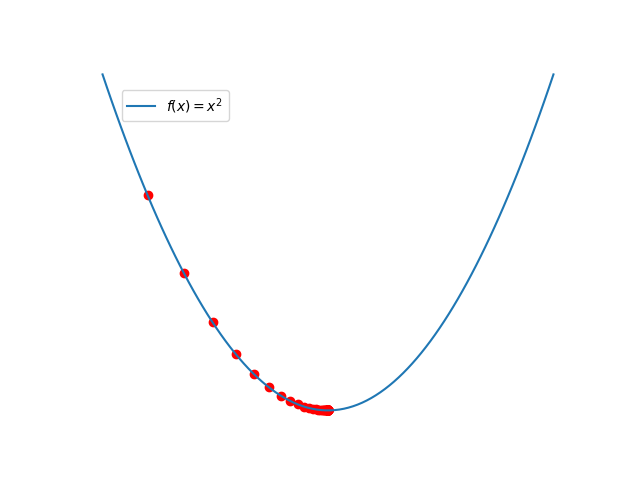
\includegraphics[width=0.68\textwidth]{Project2/figures/simple_gradient_descent.png}
    \caption{Gradient Descent | $\eta = 0.01$, $w_0 = -4$, 100 iterations}
    \label{fig:simple_gradient_descent}
\end{figure}
For this simple example the iteration converged quickly, reaching a absolute value less than 0.001 after only 27 iterations. Gradient descent is not always this efficient. 

The two natural weaknesses of gradient descent are neatly explained in \cite[p.~65--71]{MLRefined}. The first stems from the gradient being always perpendicular to the contour line. This is easily proved through parameterization.


\begin{lemma}
    Let $w(t)$ be a parametrization of a countour surface for a differentiable function $f: X^n \rightarrow Y$. Then $\nabla f \perp w(t) $ 
\end{lemma}

\begin{proof}
$$f(w(t)) = C \Rightarrow \frac{d}{dt} f(w(t)) = 0 \Rightarrow \nabla f(w(t)) \cdot \frac{\partial w(t)}{\partial t} = 0$$
The result follows from $\frac{\partial w(t)}{\partial t}$ being parallel to the contour
\end{proof}

This may lead to Zig-zagging behavior for ill conditioned problems.

\begin{figure}[H]
    \centering
    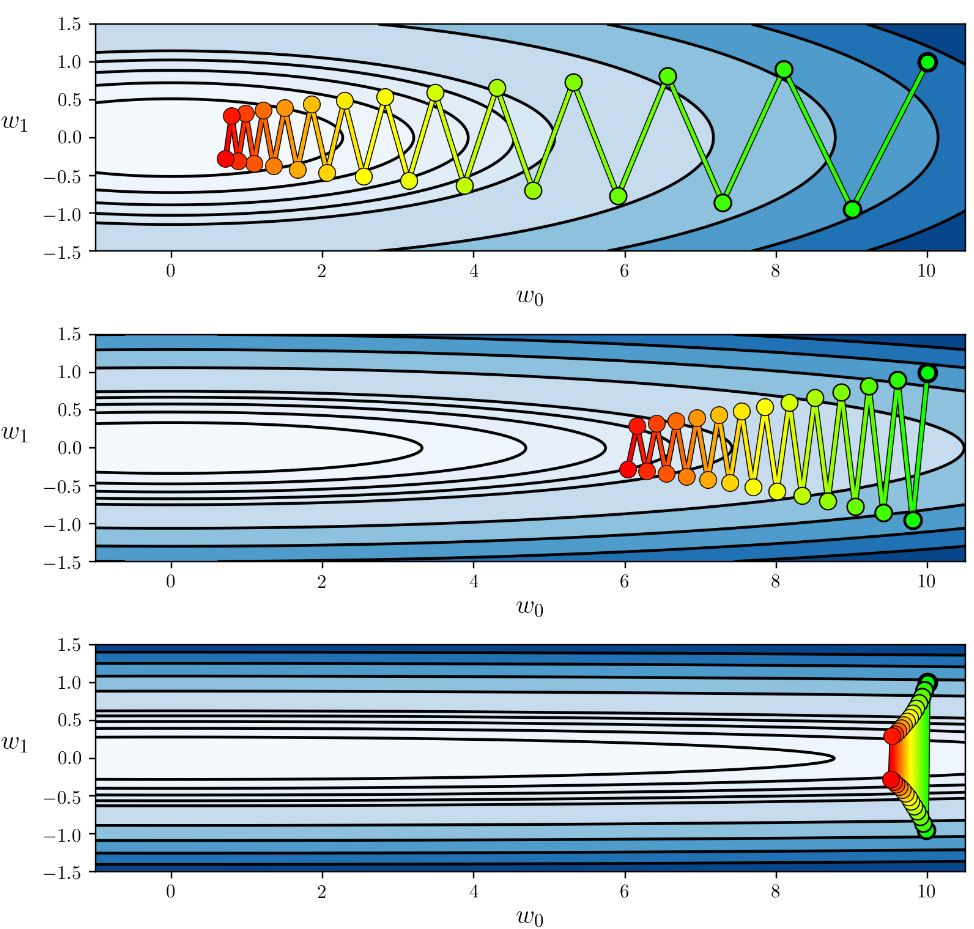
\includegraphics[width=0.9\textwidth]{Project2/figures/Gradient_descent_zigzag.jpeg}
    \caption{Figure 3.13 \cite[p.~68]{MLRefined} illustrating the zig-zagging behavior
of gradient descent.}
    \label{fig:zigzagGradientDescent}
\end{figure}

The other challenge of gradient descent is its slow crawling behaviour in flatter regions of a function such as saddle points.  
This is nicely illustrated by 50 iterations with $\eta = 0.1$ on the function 
\[g(w) =  max^2(0, 1 + (3w - 2.3)^3) + max^2(0, 1 + (-3w + 0.7)^3)\]

\begin{figure}[H]
    \centering
    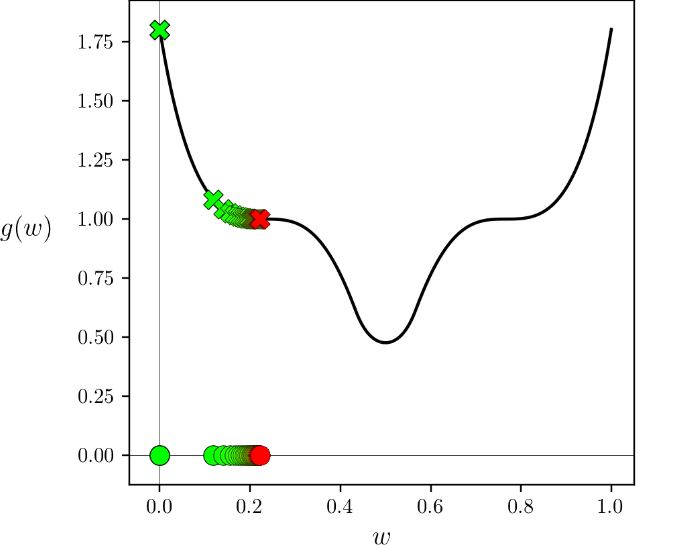
\includegraphics[width=0.7\textwidth]{Project2/figures/Gradient_descent_saddle_crawl.jpeg}
    \caption{Figure 3.14 \cite[p.~70]{MLRefined} illustrating the slow crawling behaviour
of gradient descent.}
    \label{fig:CrawlGradientDescent}
\end{figure}

\subsubsection{Stochastic gradient descent}
Stochastic gradient descent (or SGD) introduces the concept of batching. Instead of computing the gradient for all data points, as is done in deterministic gradient descent, we split the data set into batches (or mini-batches). \\
Let $M$ be the size of the batches and $n$ the number of data points, then the number of batches will be $m = \frac{M}{n}$. In the special case of $M = n$, there is only one batch and SGD becomes "vanilla" gradient descent again. In SGD, the algorithm have an inner loop that iterates $m$ times. For each time a new batch is drawn randomly from the data points and calculates the gradient and updates the learning rate. \\
Let $\mathbf{x_i}$ be the $i_{th}$ batch and $i=1,...,m$, then we can rewrite eq. \ref{eq:1} as
\begin{equation*}
        \mathbf{w_{j+1}} = \mathbf{w_j} - \eta_k\nabla\mathbf{f(x_i)}
\end{equation*}
where $j=1,...,m+epochs$. As stated above, the gradient descent finds the local minima $f(\xi)$ by exploitation. This is beneficial for convex functions or if the local minima is already known to be the global minima. For non-convex functions or in the case where the global minima is not known (which is the case most of the time), SGD introduces more exploration. This means that instead of getting stuck in a local minima, by randomness, there is a higher probability of finding the global minima. SGD also have an added bonus that it is dependent on the batch size rather than the data set size. Thus the learning rate can still converge, even if the data set gets large.

\subsubsection{Momentum based gradient descent}
Momentum is an added parameter meant to address these issues of vanilla gradient descent. The iteration is defined as

\begin{align*}
    \mathbf{w_{k+1}} &= \mathbf{w_k} + \mathbf{v_{t+1}}, \\
    \mathbf{v_{t+1}} &= \rho \mathbf{v_t} - \eta\mathbf{\nabla f(w_k)}, \hspace{3mm} \mathbf{v_0} = 0
\end{align*}

$\mathbf{v}$ is called the velocity term and $\rho$ is the momentum parameter. $\rho$ can be thought of as the velocities resistance to change while the learning rate ($\eta$) characterizes the influence of the gradient. An intuitive analogy is to think of our descent algorithm as a particle moving on the surface we wish to minimize. The gradient is the force acting on our particle ($\eta$ is its amplifier) and $\rho$ is the mass of the particle. This way our particle might be able to roll past the saddle point in Figure \ref{fig:CrawlGradientDescent} and obtain a less "zig-zaggy" path in Figure \ref{fig:ZigZagMomentumGradientDescent}.

\newpage

Here we see momentum gradient descent performed on the same ill conditioned problem as the first panel of Figure \ref{fig:ZigZagMomentumGradientDescent} with $\rho$ equal to $0, 0.2, 0.7$ respectively

\begin{figure}[H]
    \centering
    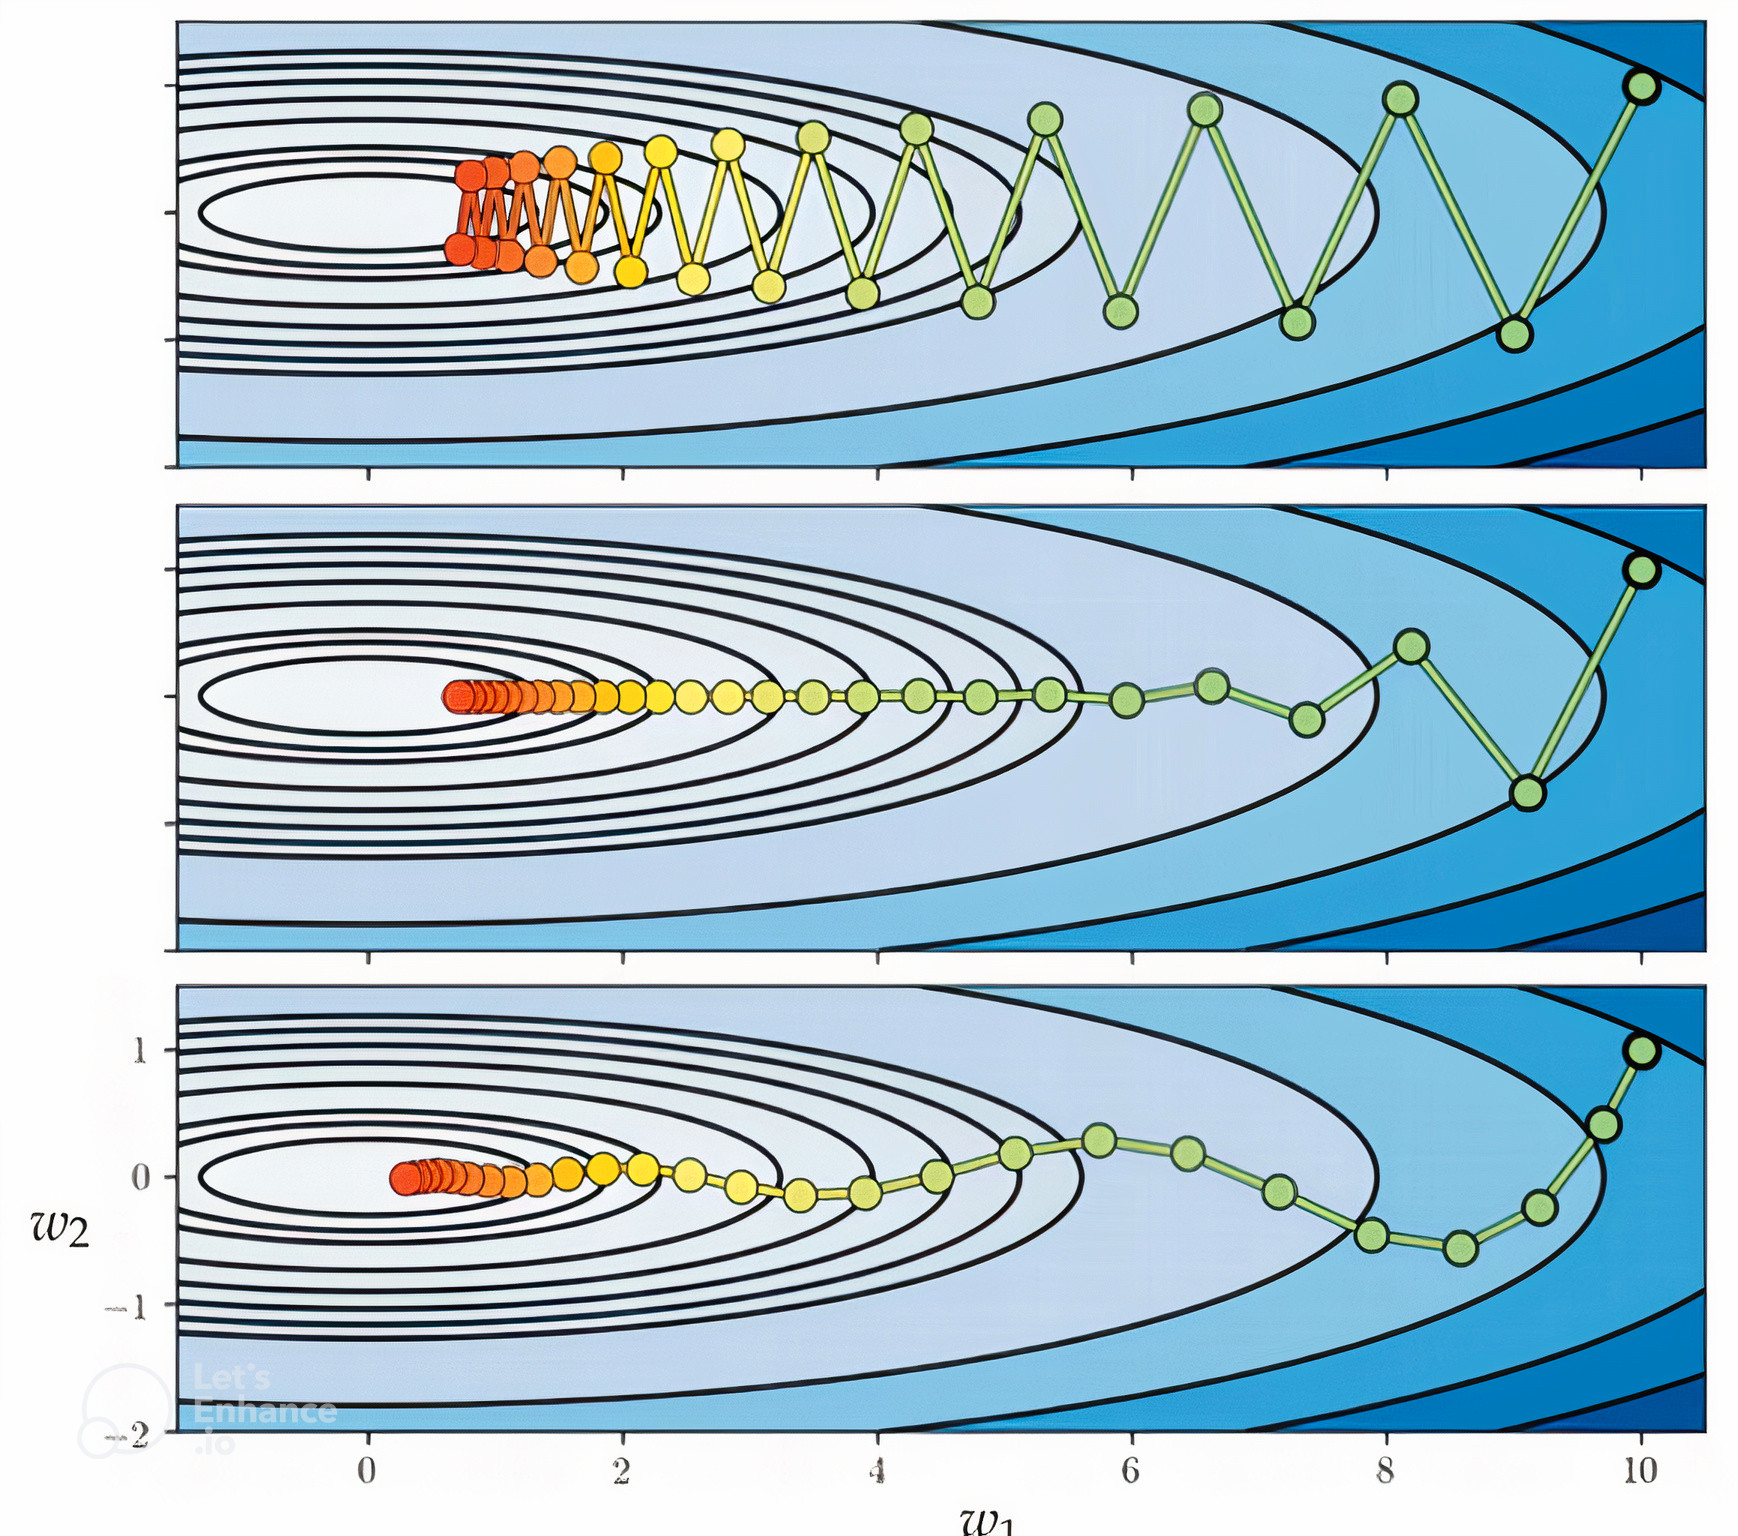
\includegraphics[width=0.8\textwidth]{Project2/figures/momentum_based_gradient_descent_less_zig.jpg.jpg}
    \caption{Figure A3 \cite[p.~478]{MLRefined} The zig-zagging behavior of gradient
descent can be ameliorated using the momentum-accelerated gradient descent}
    \label{fig:ZigZagMomentumGradientDescent}
\end{figure}


\subsubsection{AdaGrad}
The Adaptive gradient optimizer, commonly referred to as AdaGrad was introduced by \cite{duchi2011adaptive} and its update rule is given by

\[ w_{k+1}= w_{k}-\eta G_{k}^{-1/2} \odot \nabla f(w_k) \]
where $\odot$ is the harmand product, $G_k$ is the diagonal of the outer product of all previous subgradients
\[
G_k = diag\left(\sum_{i = 0}^k \nabla f(w_i) \nabla f(w_i)^T\right)
\]
 Essentially  $G_{k,i}$ ( the $i$-th component of $G_k$) is the sum of the squares of the previous gradients in direction $i$

 Normally a small numerical stabiliser is added to $G_k$ to avoid division by zero
 \[
 w_{k+1}= w_{k}-\eta \left(\delta G_{k}\right)^{-1/2} \odot \nabla f(w_k)
 \]
 Element wise the update looks like this
 \[
 \begin{bmatrix}w_{k+1}^{(1)}\\w_{k+1}^{(2)}\\\vdots \\w_{k+1}^{(m)}\end{bmatrix}={\begin{bmatrix}w_{k}^{(1)}\\w_{k}^{(2)}\\\vdots \\w_{k}^{(m)}\end{bmatrix}}-{\begin{bmatrix}\eta {\frac {1}{\sqrt {\epsilon +G_{k}^{(1)}}}}\\\eta {\frac {1}{\sqrt {\delta  +G_{k}^{(2)}}}}\\\vdots \\\eta {\frac {1}{\sqrt {\delta +G_{k}^{(m)}}}}\end{bmatrix}}\odot \begin{bmatrix}\nabla f(w_k)^{(1)}\\\nabla f(w_k)^{(2)}\\\vdots \\\nabla f(w_k)^{(m)}\end{bmatrix}
 \]

Note that as $G_k^{(i)}$ grows the step size in direction $i$ decreases. This means that the algorithm places less emphasis on a particular direction after having traversed it. This is the core idea behind AdaGrads design. Adagrad thus works well under the assumption that we need to move about the same distance in each dimension. It also enjoys a decaying step size, which is beneficial if we reach our minima, but could mean that our algorithm grinds to a halt, before reaching it, if $\eta$ is to small.

\subsubsection{RMSprop}
RMSprop, root mean square propagation, was first introduced in 2018, in lecture 6 of the Coursera course "Neural Networks for Machine Learning" by Geoff Hinton
\cite{NNforML-Lecture6}
\subsubsection{ADAM}


\subsection{Neural Networks}
Neural networks are computational systems loosely based on networks of neurons in the brain. \\
... \\
A neural network mainly consists of an input layer of nodes, a set of weights, an activation function, a hidden layer of nodes and a layer of output nodes. The input nodes are usually called features. Each node is connected to all nodes in the next layer and the edge between them have a weight on it. In the next layer, each input to the node is multiplied with its own weight and then summed together. These nodes are usually what we would call an artificial neuron.\\
Let $f: X \rightarrow Y$ be a function (?), then we can define the artificial neuron as
\begin{equation*}
    y = f(\sum_{i=1}^{n}w_ix_i)
\end{equation*}


\subsubsection{Activation functions}

\subsubsection{Back propagation}

\section{Method}

\section{Results}

\section{Discussion}

\section{Conclusion}

\section{References}

\bibliography{Project2/refs} % add  references to this 

\section{Appendix}
The code is publicly available on \href{https://github.com/augustfe/FYSSTK}{github.com/augustfe/FYSSTK}, written in python.


\end{document}